%\documentclass[tikz,svgnames,border={0 2}]{standalone}
\renewcommand\vec[1]{\boldsymbol{#1}}

%\begin{document}
\begin{tikzpicture}[
    box/.style={rectangle,draw,fill=DarkGray!20,node distance=1cm,text width=15em,text centered,rounded corners,minimum height=2em,thick},
    arrow/.style={draw,-latex',thick},
  ]

  \node [box] (potential) {$v_{\text{ext},s}(\vec r)=v_\text{H}(\vec r) + v_\text{xc}(\vec r) + v_\text{ext}(\vec r)$};
  \node [box,below=0.5 of potential] (hamiltonian) {$\hat{H}_{KS}=-\frac{\hbar^2}{2m}\vec{\nabla}^2 + v_{\text{ext},s}(\vec r)$};
  \node [box,below=0.5 of hamiltonian] (se) {$\hat{H}_{KS} \phi_i(\vec r)= E_i \phi_i(\vec r)$};
  \node [box,below=0.5 of se] (density) {$\rho(\vec r)=\sum_{i=1}^n f_i\,|\phi_i(\vec r_i)|^2$};
  \node [box,below=0.5 of density] (criterion) {Convergence criterion satisfied?};

%%%%%% ------------ 定义 虚线方框转角 -----------------  %%%%%%
  \path
  (potential.north west) ++(-1em,1em) coordinate (potential fit)
  (criterion.south east) ++(1em,-1em) coordinate (criterion fit);

  \node [box,above=1.5 of potential, fill=orange!30, text width=20em] (initial) {Supply initial density guess $\rho_\text{ini}(\vec r)$ to Kohn Sham equations};
  \node [box,below=1.5 of criterion, fill=blue!30, text width=20em] (energy) {Use $\rho_\text{fin}(\vec r)$ to minimize total energy functional $E_{V_\text{ext}}[\rho]=T_{e,s}[\phi_i\{\rho\}] + V_{ee,H}[\rho] + E_{xc}[\rho] + V_{eI}[\rho]$};

  \path [arrow] (initial) -- (potential);
  \path [arrow] (potential) -- (hamiltonian);
  \path [arrow] (hamiltonian) -- (se);
  \path [arrow] (se) -- (density);
  \path [arrow] (density) -- (criterion);

%%%%%% ------------ 绘制 虚线方框 -----------------  %%%%%%
  \node [rectangle,draw,dashed,inner sep=1em,fit=(potential fit) (criterion fit)] (enclosure) {};
  \node [above=-0.8em of enclosure,anchor=south,draw,outer sep=0pt,fill=white] (enclosure label) {\Large\textbf{Kohn-Sham method}};

  \path [arrow] (criterion) -- (energy) node [midway,left=0.1,draw,outer sep=0pt,fill=white] (TextNode) {Yes};
  \path [draw,thick] (criterion.south) ++(0em,-1em) -- (criterion fit) node [midway,below=0.1,sloped,draw,outer sep=0pt,fill=white] (TextNode) {No};
  \draw [arrow] (criterion fit) |- (potential.east);

\end{tikzpicture}

\begin{tikzpicture}

  % Define radius
  \def\r{3}

  % Bloch vector
  \draw (0, 0) node[circle, fill, inner sep=1] (orig) {} -- (\r/3, \r/2) node[circle, fill, inner sep=0.7, label=above:$\vec{a}$] (a) {};
  \draw[dashed] (orig) -- (\r/3, -\r/5) node (phi) {} -- (a);

  % Sphere
  \draw (orig) circle (\r);
  \draw[dashed] (orig) ellipse (\r{} and \r/3);

  % Axes
  \draw[->] (orig) -- ++(-\r/5, -\r/3) node[below] (x1) {$x_1$};
  \draw[->] (orig) -- ++(\r, 0) node[right] (x2) {$x_2$};
  \draw[->] (orig) -- ++(0, \r) node[above] (x3) {$x_3$};

  % Angles
  \pic [draw=gray, text=gray, ->, "$\phi$"] {angle = x1--orig--phi};
  \pic [draw=gray, text=gray, <-, "$\theta$", angle eccentricity=1.4] {angle = a--orig--x3};

\end{tikzpicture}
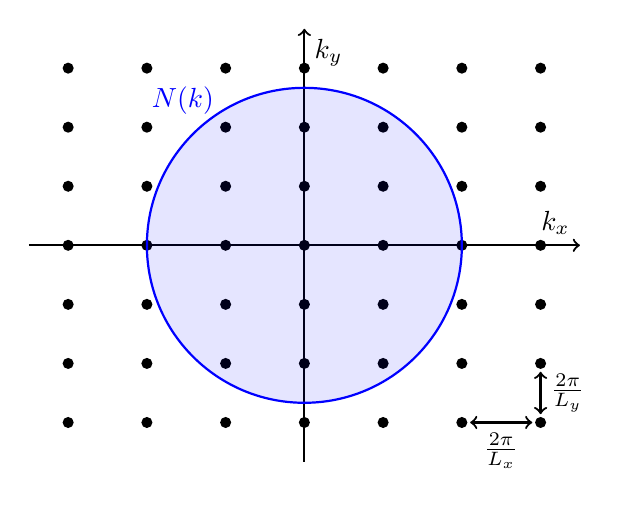
\begin{tikzpicture}[thick]

  % Dot grid
  \def\xrange{3}
  \def\yrange{3}
  \def\ratio{3/4}
  \foreach \x in {-\xrange,...,\xrange}
    {\foreach \y in {-\yrange,...,\yrange}
        {\fill (\x,\ratio*\y) circle[radius=2pt];}}

  % Axes
  \draw[->] (-\xrange-1/2,0) -- (\xrange+1/2,0) node[above left] {$k_x$};
  \draw[->] (0,-\ratio*\yrange-1/2) -- (0,\ratio*\yrange+1/2) node[below right] {$k_y$};

  % Lattice spacing
  \draw[<->,shorten >=3,shorten <=3] (\xrange-1,-\ratio*\yrange) -- (\xrange,-\ratio*\yrange) node[midway,below] {$\frac{2 \pi}{L_x}$};
  \draw[<->,shorten >=3,shorten <=3] (\xrange,-\ratio*\yrange) -- (\xrange,-\ratio*\yrange+\ratio) node[midway,right] {$\frac{2 \pi}{L_y}$};

  % Circle
  \draw[blue,fill=blue,fill opacity=0.1] (0,0) circle (2/3*\yrange);
  \node[blue] at (130:2.4) {$N(k)$};
\end{tikzpicture}

\begin{tikzpicture}[
    g/.style={rectangle,draw,rounded corners,minimum height=6em,inner sep=1em,font=\Huge},
    w/.style={font=\Huge},
    c/.style={node distance=15ex,align=left,font=\huge},
    a/.style={draw,-latex',ultra thick}
  ]

  \node [w,scale=3] (bra) {(};
  \node [node distance=0ex,fill=orange!30,g,right=of bra] (kinetic) {$-\frac{\hbar^2}{2m}\,\vec{\nabla}_{\vec{r}}^2$};
  \node [node distance=2ex,w,right=of kinetic] (plus1) {$+$};
  \node [node distance=2ex,fill=red!30,g,right=of plus1] (external) {$v_\text{ext}(\vec{r})$};
  \node [node distance=2ex,w,right=of external] (plus2) {$+$};
  \node [node distance=2ex,fill=red!30,g,right=of plus2] (hartree) {$v_H(\vec{r})$};
  \node [node distance=2ex,w,right=of hartree] (plus3) {$+$};
  \node [node distance=2ex,fill=red!30,g,right=of plus3] (xc) {$v_{xc}$};
  \node [node distance=0ex,w,right=of xc,scale=3] (ket) {)};
  \node [node distance=0ex,fill=gray!30,g,right=of ket] (phi1) {$\phi_i(\vec{r})$};
  \node [node distance=4ex,w,right=of phi1] (equal) {$=$};
  \node [node distance=4ex,fill=blue!30,g,right=of equal] (energy) {$E_i$};
  \node [node distance=2ex,fill=gray!30,g,right=of energy] (phi2) {$\phi_i(\vec{r})$};

  \node [c,above=of kinetic,xshift=5em] (kinetic comment) {non-rel. Schrödinger equation\\or relativistic Dirac equation};
  \node [c,below=of external,xshift=-10em] (external comment) {crystal ions or\\pseudopotential};
  \node [c,below=of hartree,xshift=5em] (hartree comment) {Poisson equation\\or Hartree potential};
  \node [c,above=of xc,xshift=-11em] (xc comment) {LDA or GGA\\or hybrids};
  \node [c,above=of phi1,xshift=5em] (phi comment) {physical orbitals or not\\mesh density and basis set};
  \node [c,below=of energy] (energy comment) {band structure\\ or not};

  \path [a] (kinetic comment) -- (kinetic.north);
  \path [a] (external comment) -- (external.south);
  \path [a] (hartree comment) -- (hartree.south);
  \path [a] (xc comment) -- (xc.north);
  \path [a] (phi comment) -- (phi1.north);
  \path [a] (phi comment) -- (phi2.north);
  \path [a] (energy comment) -- (energy.south);

\end{tikzpicture}
%\end{document}
